\documentclass[11pt]{article}
\usepackage{graphicx}
\usepackage{amssymb}
\usepackage{epstopdf}
\DeclareGraphicsRule{.tif}{png}{.png}{`convert #1 `dirname #1`/`basename #1 .tif`.png}

\textwidth = 6.5 in
\textheight = 9 in
\oddsidemargin = 0.0 in
\evensidemargin = 0.0 in
\topmargin = 0.0 in
\headheight = 0.0 in
\headsep = 0.0 in
\parskip = 0.2in
\parindent = 0.0in

\newtheorem{theorem}{Theorem}
\newtheorem{corollary}[theorem]{Corollary}
\newtheorem{definition}{Definition}

\title{QuERI Front-end Schematics}
\author{John Doty, Noqsi Aerospace Ltd}
\begin{document}
\maketitle

\section{Detector Board (one page)}
The Detector Board adapts the detector to a plug on the Preamplifier Board. Its only electrical components are connectors. There is one detector board for each detector.
\section{Preamplifier Board (one page)}

The preamplifier, $U_1$, is configured for a gain of 3. With the nominal 1.8\ $\mu$V/eV detector responsivity, its output is 5.6\ $\mu$V/eV. Bias from $+2B$ (actually 1.92\ V) makes the output 2\ V (the $DUMP$ threshold) for a detector output slightly less than its nominal maximum 2\ V.

$U_2$ and $U_3$ provide regulated power for the detector and bias for the preamplifier. $R_2$, $R_3$, $C_8$, and $C_9$ filter the detector bias voltage. $D1$ senses the board temperature.

$J_1$ is the preamplifier output.

$J_2$ provides power for the preamplifier and detector. It also connects the detector and preamplifier temperature sensors.

$J_3$ connects to the detector board.

\section{Measurement/Power Unit (MPU) (16 pages)}

The MPU is organized around an A3PE3000-FG484 ProASIC FPGA. For clarity, this is divided in the schematic into 14 subsystems, $U_{1A}$-$U_{1N}$. Each FPGA subsystem is drawn on the page where its function resides.

The MPU power, control, and signal processing for two Focal Plane Modules (FPMs). It also controls a Modulated X-ray Source (MXS).

\subsection{Page 1: MPU Top Level}

\begin{table}[htp]
\caption{MPU Connectors}
\begin{center}
\begin{tabular}{|l|l|}
\hline
Connector & Function \\
\hline
\hline
J1 & X-ray pulses from FPM 0 \\
J2 & X-ray pulses from FPM 1 \\
J3 & Power and temperature monitoring for FPM 0 \\
J4 & Power and temperature monitoring for FPM 1 \\
J5 & 28V power input \\
J6 & Commands and data using RS422, pulse per second using LVDS \\
J7 & Commands and data using SpaceWire \\
J8 & FPGA programming (JTAG) \\
J10 & Debugging, no fixed function \\
J13 & MXS control and monitoring \\
VP1 & FPGA flash programming voltage \\
\hline
\end{tabular}
\end{center}
\label{connectors}
\end{table}

\subsection{Page 2: X-ray channel 0}

$U_{4A}$ buffers the preamp output to the pulse shapers. $U_{3A}$ senses when the preamplifier output exceeds $VHS$ (2\ V) and signals $FULL$ to logic when it does. $U_{3B}$ when the unipolar output of the slow shaper exceeds the full range of the circuitry ($VFS$, 4\ V) and signals $OVER$ to logic when it does. $U_{4B}$ buffers the 2.5\ V reference.

$U_{6A}$ regulates the current to the detector's thermoelectric cooler via $Q_1$. $U_{6B}$ senses the current for housekeeping.

$U_5$, $Q_2$, and $Q_3$ are the regulation loop for the detector bias voltage. $U_{5B}$ converts the output voltage range 0 to -160\ V to 0 to 4\ V for housekeeping and regulation. $U_{5A}$ compares that converted voltage to the commanded $HVDAC$ voltage. R34 converts the error voltage out of $U_5A$ to a current. The error current is relayed to the high voltage section of the circuit via $Q_2$. It develops a voltage against $R_{35}$, which feeds the base of pass transistor $Q3$. $R_{36}$ and $C_{14}$ provide the dominant pole stabilizing the loop, along with some noise filtering.

\subsection{Page 3: Fast Shaper}
The 
\begin{figure}[htbp]
\begin{center}
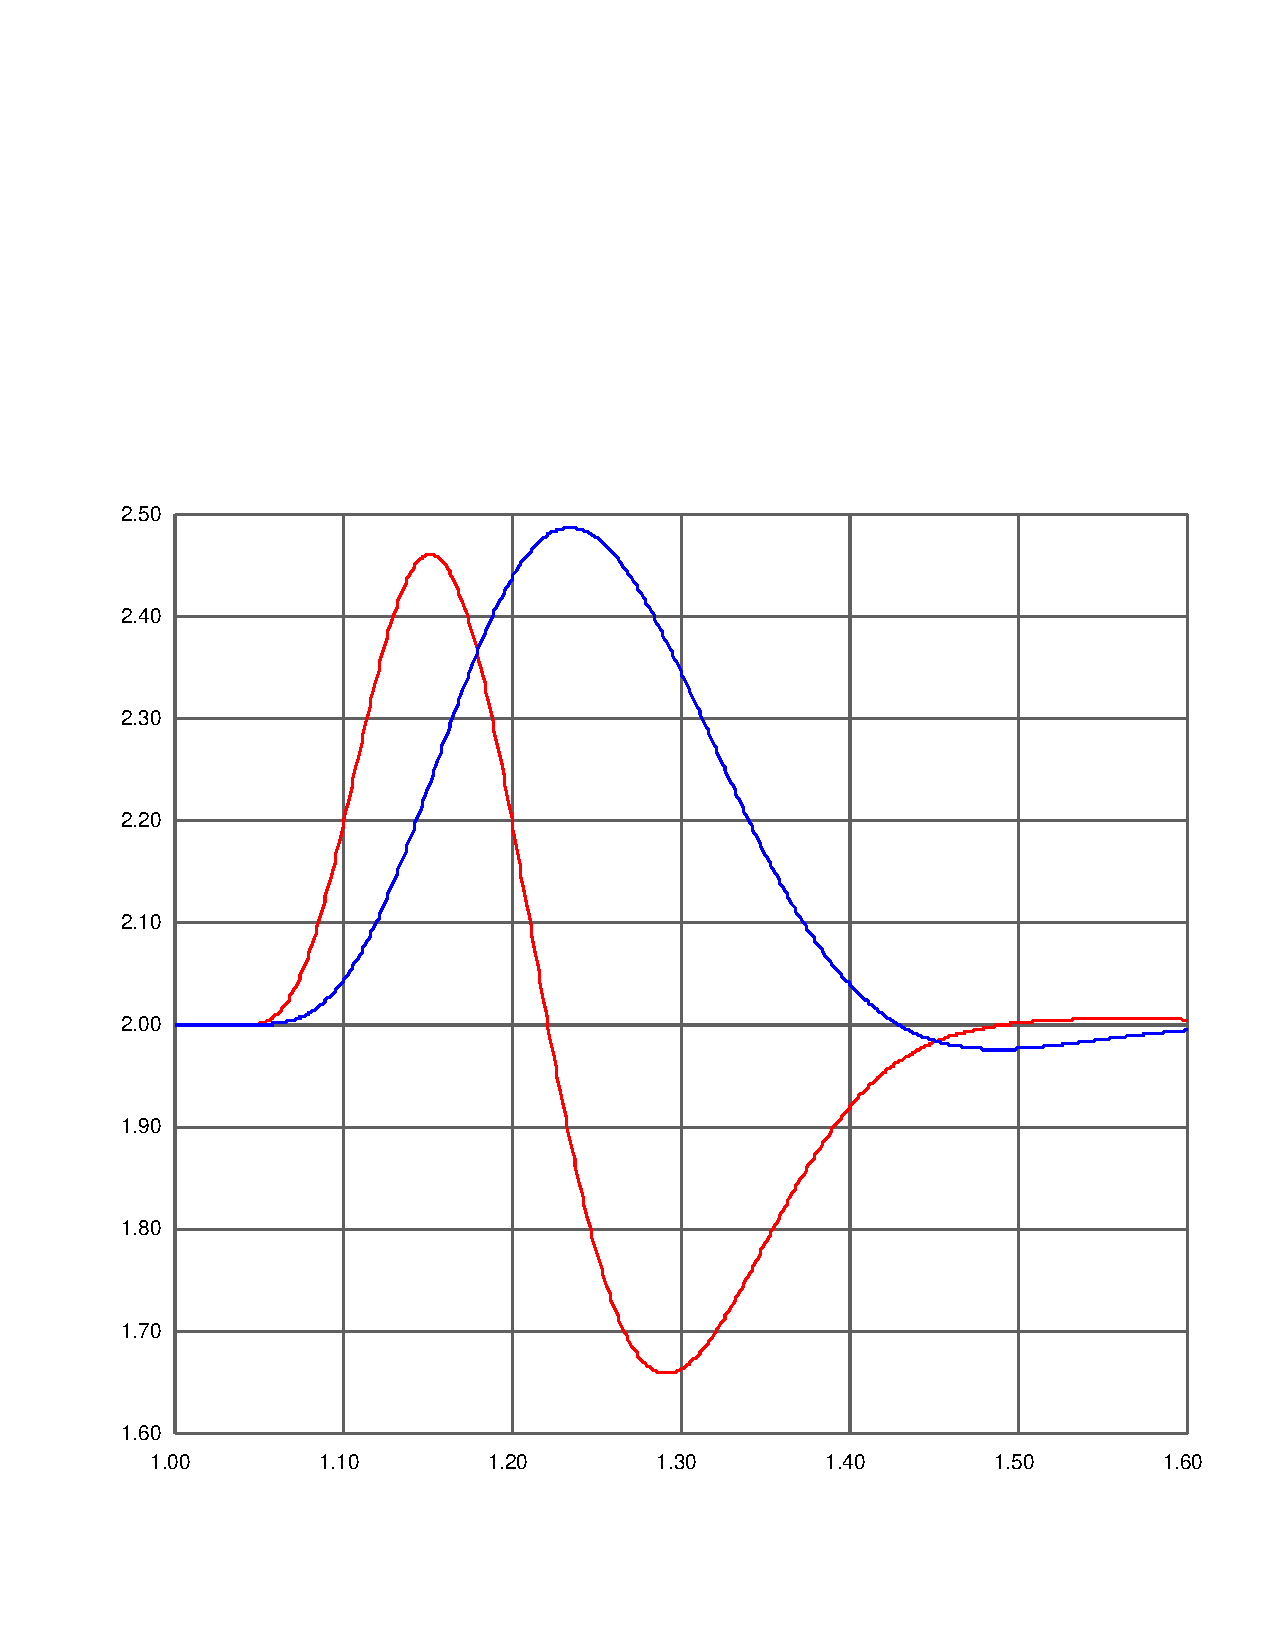
\includegraphics{FastShaping.pdf}
\caption{Simulated Fast Shaper outputs for a 54\ mV edge, equivalent to a 10\ keV x-ray. Horizontal axis is time in $\mu$s, vertical is volts. Blue is the $UNIPOLAR$ output, blue is $BIPOLAR$. The edge had a linear 10\ ns rise starting at 1\ $\mu$s.}
\label{FastShaping}
\end{center}
\end{figure}




\end{document}
